\documentclass{beamer}
\usepackage{graphicx}
\usepackage{paralist}
\usepackage{outlines}

\title{Text, Styles, Fill and Adjustment Layers}
\author{Joshua Paul Barnard}
\titlegraphic{\vspace{-10mm}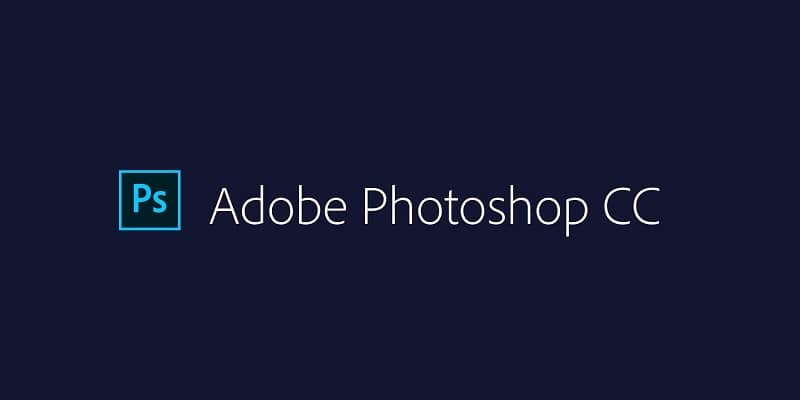
\includegraphics[width = .8\textwidth]{images/photoshop.jpg}} 
\date{\vspace{-5em}} 


\mode <presentation>
\usetheme{Warsaw}
\usecolortheme{default}

\setbeamerfont{footline}{size=\fontsize{5}{8}\selectfont}

\definecolor{darkred}{rgb}{20,0,0}
\definecolor{darkgreen}{RGB}{40,110,20}
\definecolor{darkpurple}{RGB}{30,0,30}
\definecolor{chardonnay}{RGB}{255, 255, 204}

\setbeamercolor*{palette primary}{fg=white, bg=darkgreen}


\begin{document}
	{
		\setbeamertemplate{footline}{} 
		\setbeamertemplate{headline}{} 
		\begin{frame}
			\vspace{-35pt}
			\maketitle
		\end{frame}
	}

	\section{}	
\subsection{Table of Contents - Week 3}
\begin{frame}
	\frametitle{Table of Contents - Week 3}
	\begin{columns}
		\column{.6\textwidth}
		\vspace{-25pt}
		\begin{itemize}
			\item Creating a New Project
			\item Fill and Adjustment Layers
			\item The Type Tool
			\item Layer Styles
			\item The Snipping Tool
		\end{itemize}
		\column{.45\textwidth}
		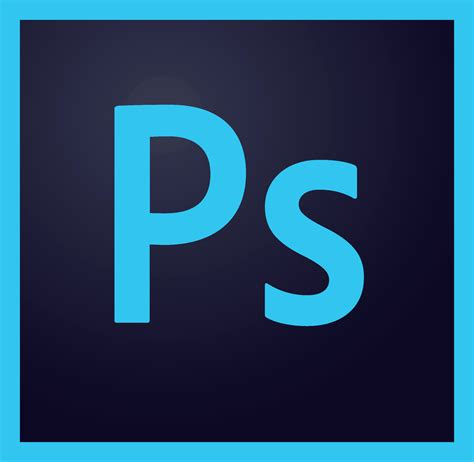
\includegraphics[width=.85\textwidth]{images/ps.jpg}
	\end{columns}
\end{frame}


	\section{Creating a New Project}
		\begin{frame}
		\frametitle{Photoshop Project Files}
		\begin{center}
			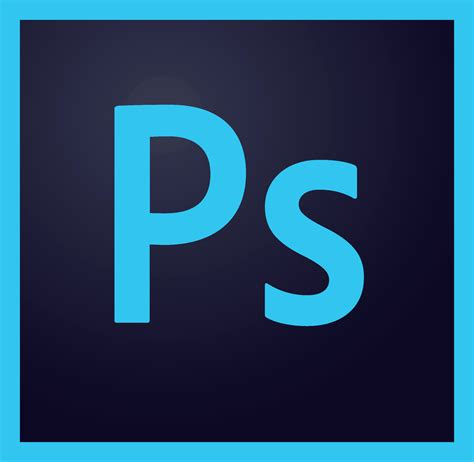
\includegraphics[width = 0.8\textwidth]{images/th.jpg}
		\end{center}
	\end{frame}
	
			\subsection{How to Create a new Photoshop Project}		
	\begin{frame}
		\frametitle{How to Create a New Photoshop Project}
	\begin{columns}
	\column{.6\textwidth}
	\vspace{-15pt}
	\begin{outline}
		\1 Open Photoshop
		\1 Click File, in the menu bar
		\1 Click New
		\1 Hotkey:  Ctrl + N
	\end{outline}
	\column{.45\textwidth}
	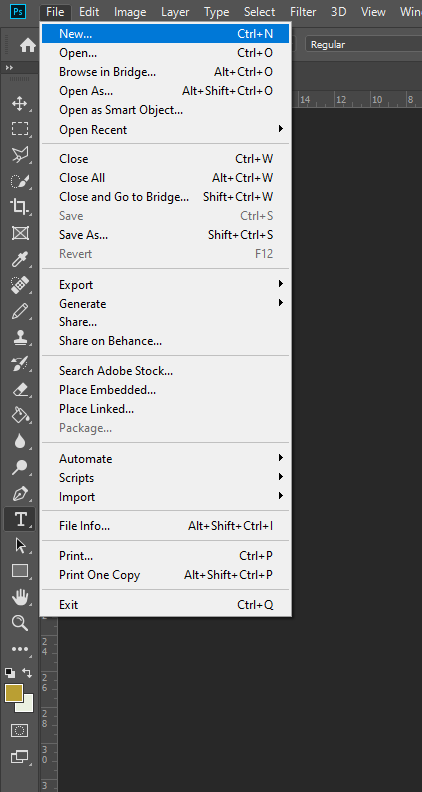
\includegraphics[width=.7\textwidth]{images/new project 1.png}
\end{columns}
		\end{frame}

\subsection{Setting up a new Photoshop Project}	
\begin{frame}
	\frametitle{Setting up a new Photoshop Project}
	\begin{outline}
		\1 You can set the initial image settings:
		\2 Name
		\2 Width and Height
		\2 Orientation
		\2 Resolution
		\2 Color Modes
	\end{outline}
	\begin{center}
		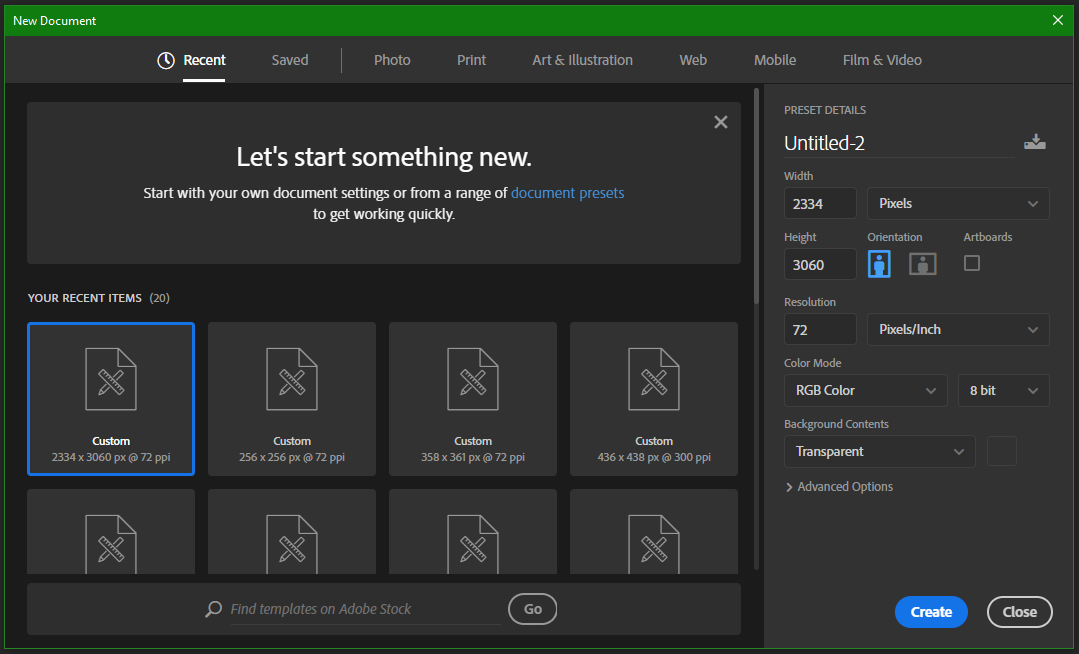
\includegraphics[width = 0.6\textwidth]{images/new project 2.png}
	\end{center}
\end{frame}
	
	
	\section{Fill and Adjustment Layers}
	\begin{frame}
		\frametitle{Fill and Adjustment Layers}
		\begin{center}
			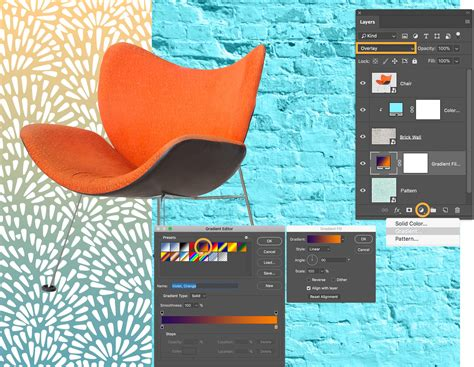
\includegraphics[width = 0.8\textwidth]{images/adjust and fill layers.jpg}
		\end{center}
	\end{frame}
	
\subsection{How to Create Fill and Adjustment Layers}
\begin{frame}
	\frametitle{How to Create Fill and Adjustment Layers}
		\begin{columns}
		\column{.6\textwidth}
		\vspace{-15pt}
	\begin{itemize}
		\item Select the layer you want to work on
		\item Click the half-filled circle in the bottom left corner of the screen to bring up your options
		\item Choose the layer you want
	\end{itemize}
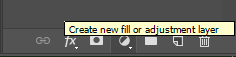
\includegraphics[width = 1.0\textwidth]{images/fill1.png}
	\column{.45\textwidth}
	\begin{center}
			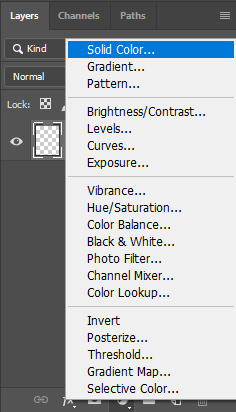
\includegraphics[width = 1.0\textwidth]{images/fill2.png}
	\end{center}
\end{columns}
\end{frame}

\subsection{Fill Layers}
\begin{frame}
	\frametitle{What are Fill Layers?}
	\begin{outline}
		\1 Fill layers let you fill a layer with a solid color, gradient, or pattern.
		\1 They do not effect the layers below them.
		\1 There are only 3 fill layers:
		\2 Solid Color...
		\2 Gradient...
		\2 Pattern...
	\end{outline}
	\begin{center}
		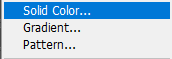
\includegraphics[width = 1.0\textwidth]{images/fill3.png}
	\end{center}
\end{frame}

\begin{frame}
	\frametitle{Solid Color...}
	\begin{outline}
		\1 Creates a layer filled with a solid color chosen from the Color Picker.
	\end{outline}
	\begin{center}
		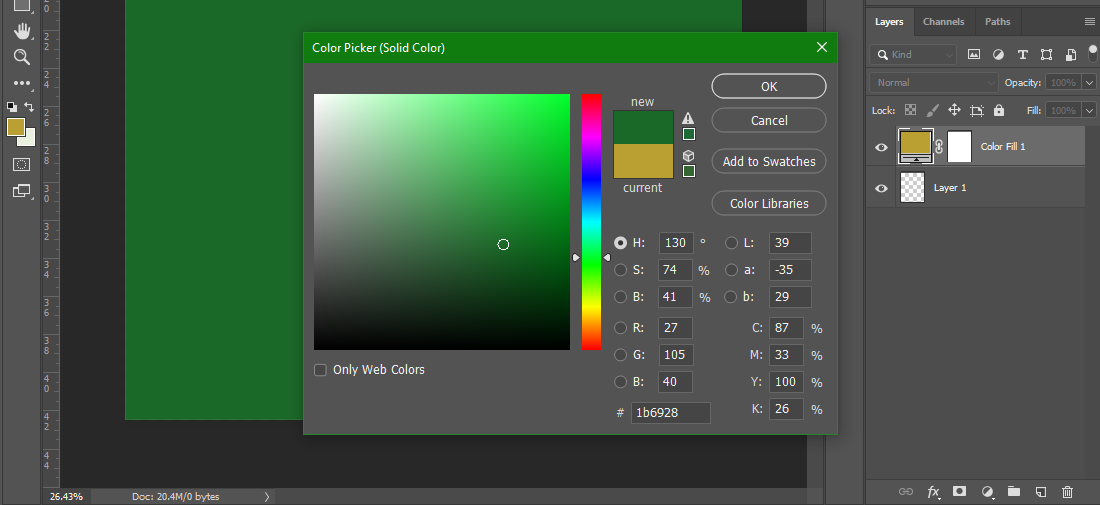
\includegraphics[width = 1.0\textwidth]{images/solid colour.png}
	\end{center}
\end{frame}

\begin{frame}
	\frametitle{Gradient...}
	\begin{outline}
		\1 Creates a layer filled with a gradient. 
		\2 You can choose a predefined gradient from the Gradient menu. 
		\3 To edit the gradient in the Gradient Editor, click the color gradient. 
		\3 You can drag within the image window to move the center of the gradient.  
		\2 You can also specify the shape of the gradient (Style) and the angle at which it is applied (Angle). 
		\2 Select Reverse to flip its orientation, Dither to reduce banding, and Align With Layer to use the layer’s bounding box to calculate the gradient fill.
	\end{outline}
\end{frame}

\begin{frame}
	\frametitle{Gradient...}
	\begin{center}
		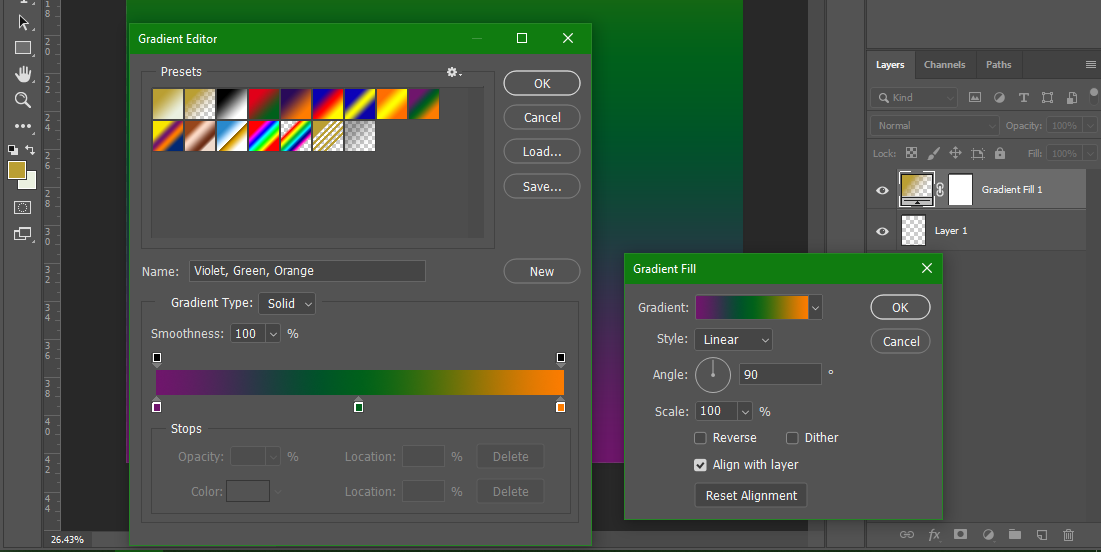
\includegraphics[width = 1.0\textwidth]{images/gradient.png}
	\end{center}
\end{frame}

\begin{frame}
	\frametitle{Pattern...}
	\begin{outline}
		\1 Creates a layer filled with a pattern. 
		\2 Click the pattern, and choose a pattern from the pop‑up panel. 
		\2 You can scale the pattern and choose Snap To Origin to position the origin of the pattern with that of the document window. 
		\2 To specify that the pattern moves with the Fill layer as it is relocated, select Link With Layer. 
		\3 When this option is selected, you can drag within the image to position the pattern while the Pattern Fill dialog box is open. 
		\2 To create a new preset pattern after editing pattern settings, click the New Preset button.
	\end{outline}
\end{frame}

\begin{frame}
	\frametitle{Pattern...}
	\begin{center}
		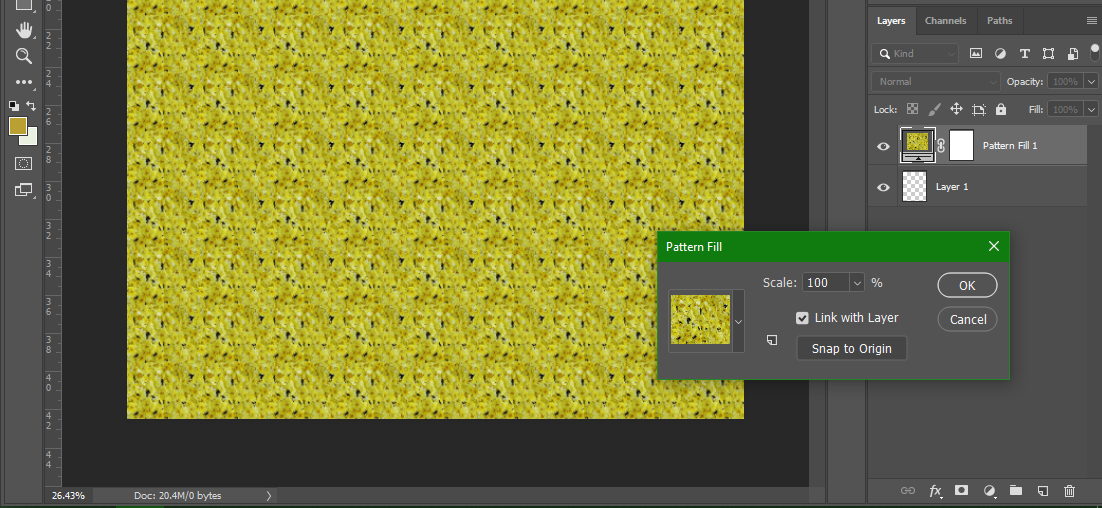
\includegraphics[width = 1.0\textwidth]{images/pattern.png}
	\end{center}
\end{frame}

\subsection{Adjustment Layers}
\begin{frame}
	\frametitle{What is an Adjustment Layer?}
	\begin{outline}
		\1 A layer that lets you apply color and tonal adjustments to your image without permanently changing pixel values.
		\1 Effects all the layers below the adjustment layer.
		\1 They provide the following benefits:
		\2 Nondestructive edits. You can try different settings and re‑edit the adjustment layer at any time. You can also reduce the effect of the adjustment by lowering the opacity of the layer.
		\2 Selective editing. Paint on the adjustment layer's image mask to apply an adjustment to part of an image. Later you can control which parts of the image are adjusted by re-editing the layer mask. You can vary the adjustment by painting on the mask with different tones of gray.
		\2 Ability to apply adjustments to multiple images. Copy and paste adjustment layers between images to apply the same color and tonal adjustments.
	\end{outline}
\end{frame}

\begin{frame}
	\frametitle{What is an Adjustment Layer?}
		\begin{center}
		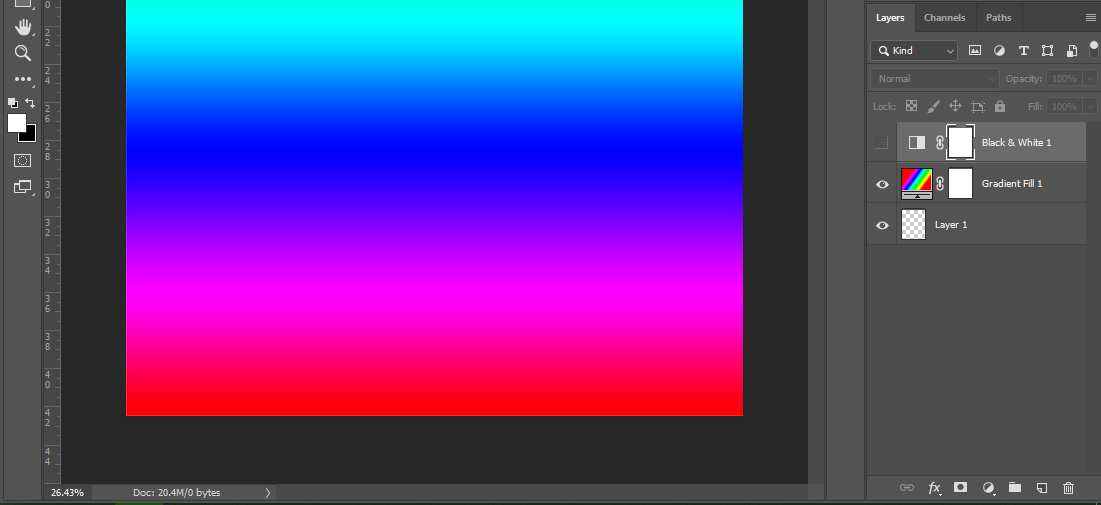
\includegraphics[width = 0.85\textwidth]{images/adjustment2.png}
	\end{center}
	\begin{center}
		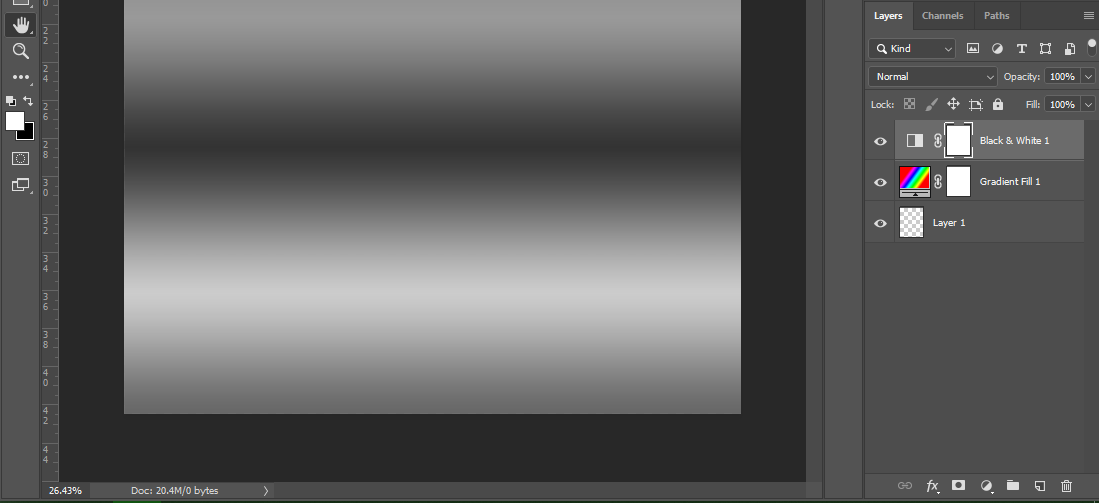
\includegraphics[width = 0.85\textwidth]{images/adjustment1.png}
	\end{center}
\end{frame}

\begin{frame}
	\frametitle{What are the Adjustment Layers?}
	\begin{itemize}
		\item Brightness/Contrast - Lightens or darkens the image.
		\item Hue/Saturation - Adjusts colors in the image.
		\item Levels - To correct the tonal range and color balance of an image by adjusting intensity levels of image shadows, midtones, and highlights. 
		\item Curves - Adjust points throughout an image’s tonal range. 
		\item Photo Filter - Adjusts the color balance and color temperature of the image.
		\item Invert - Produces a photo negative effect by creating a negative based on the brightness values of the image.
		\item Threshold - Renders the image in monochrome with no gray, so that you can locate the lightest and darkest areas.
		\item Posterize - Gives a flat, poster-like appearance to a photo by reducing the number of brightness values (levels) in the image, thus reducing the number of colors.

	\end{itemize}
\end{frame}

\begin{frame}
	\frametitle{What is an Adjustment Layer?}
	\begin{center}
	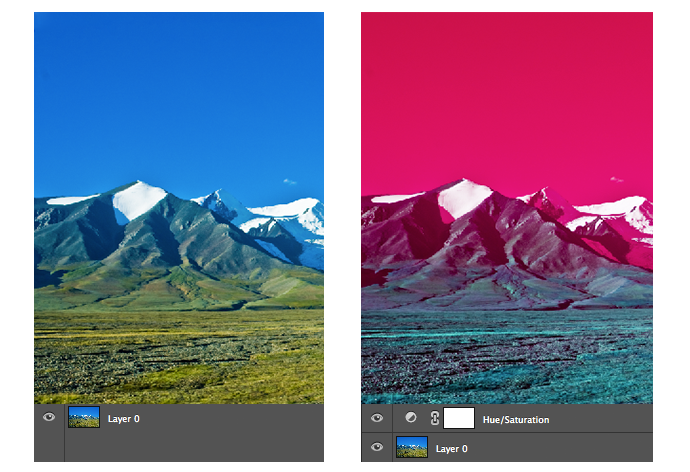
\includegraphics[width = 0.85\textwidth]{images/adjustmentLayer_PS.png}
\end{center}
\end{frame}

	\section{Type Tool}
		\begin{frame}
		\frametitle{The Type Tool}
		\begin{center}
			
\includegraphics[width = 0.8\textwidth]{images/HOW-TO-ADD-TEXT-PHOTOSHOP-THUMBNAIL.jpg}
		\end{center}
	\end{frame}
	
		\subsection{What is the Type Tool}
\begin{frame}
	\frametitle{What is the Type Tool}
	\begin{itemize}
		\item Text in Adobe Photoshop consists of vector-based type outlines.
		\item Photoshop preserves vector-based type outlines and uses them when you scale or resize type.
		\item When you create type, a new type layer is added to the Layers panel. 
		\item After you create a type layer, you can edit the type and apply layer commands to it.
	\end{itemize}
	\begin{center}
		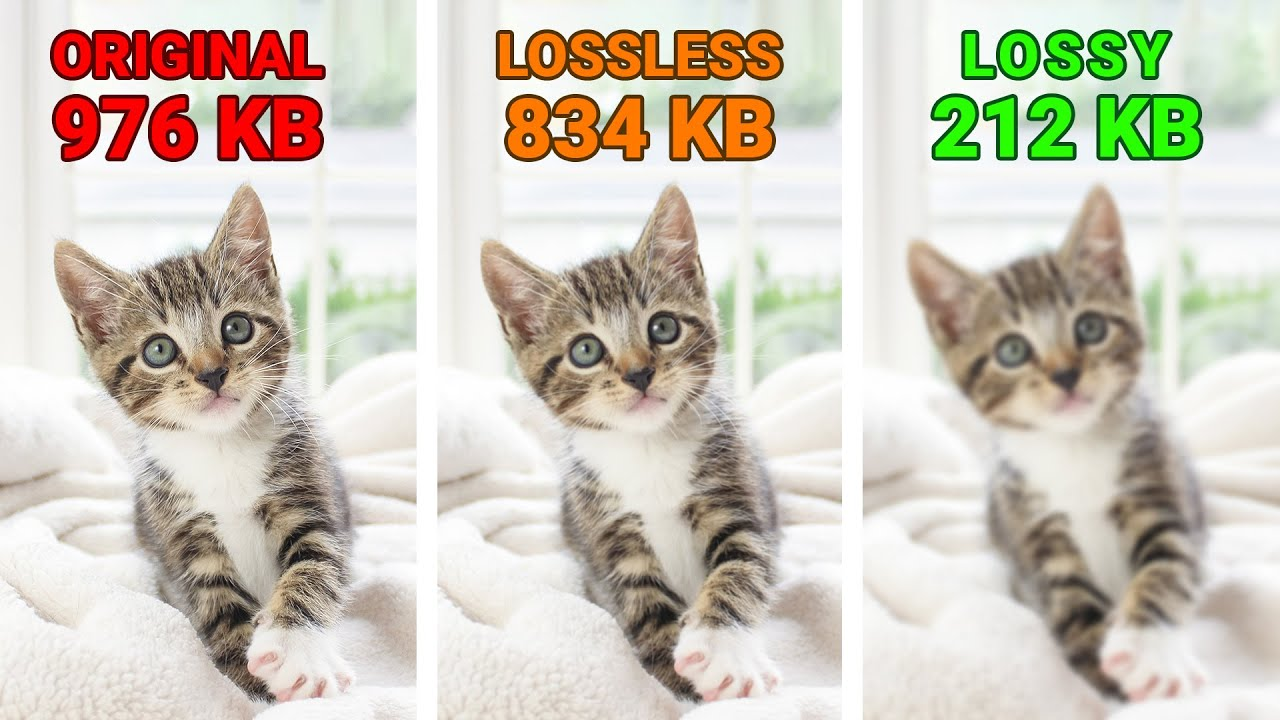
\includegraphics[width = 1.0\textwidth]{images/maxresdefault.jpg}
	\end{center}
\end{frame}

		\subsection{Type Tool}
\begin{frame}
	\frametitle{Horizontal and Vertical Type Tool}
	\begin{outline}
		\1 Select the Horizontal Type tool or the Vertical Type tool.
		\1 Click in the image to set an insertion point for the type. 
		\2 The small line through the I‑beam marks the baseline of the type (the imaginary line on which type rests). 
		\2 For vertical type, the baseline marks the center axis of the characters.
		\1 Click, hold and drag to create a section to type within. 
	\end{outline}
	\begin{center}
		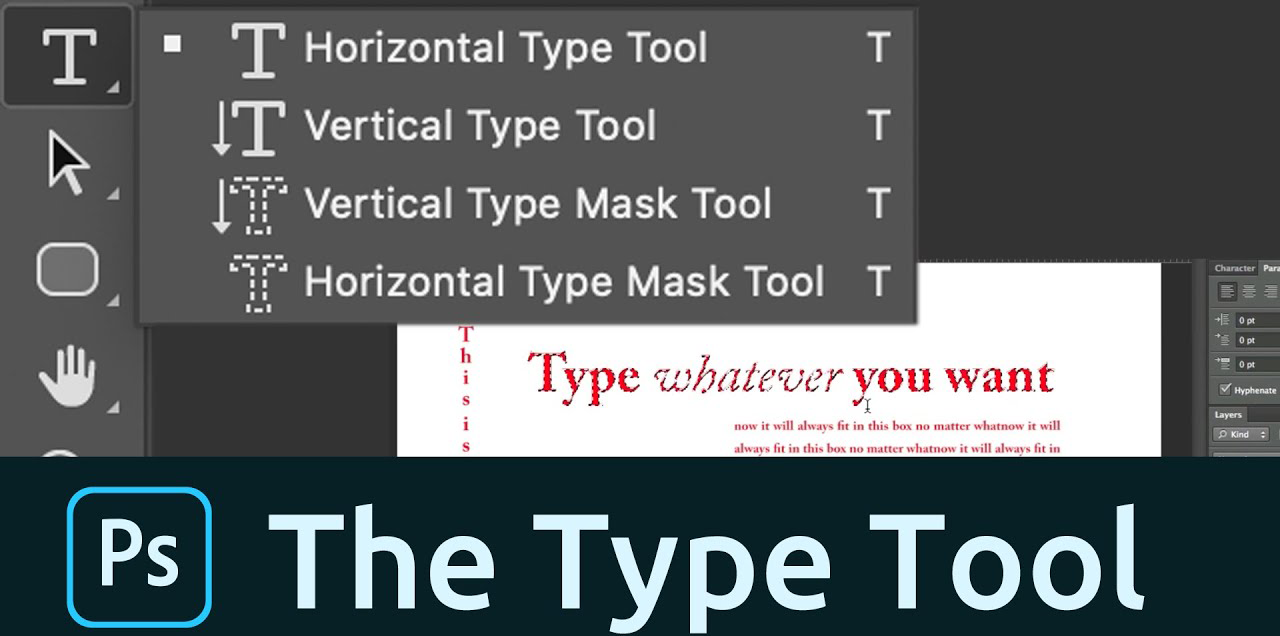
\includegraphics[width = 0.75\textwidth]{images/maxresdefault.png}
	\end{center}
\end{frame}

		\subsection{Type Mask Tool}
\begin{frame}
	\frametitle{Horizontal and Vertical Type Mask Tool}
	\begin{itemize}
		\item The Type Mask Tool permits you to cut letters out of a background.
		\item The Type Mask tool doesn't develop a new layer. Instead, it creates a selection on the active layer.
		\item This is the Tool of choice for filling up text with a picture or cutting text out of an image so that the background reveals through.
		\item We will revisit this tool after we learn about masks.
	\end{itemize}
	\begin{center}
		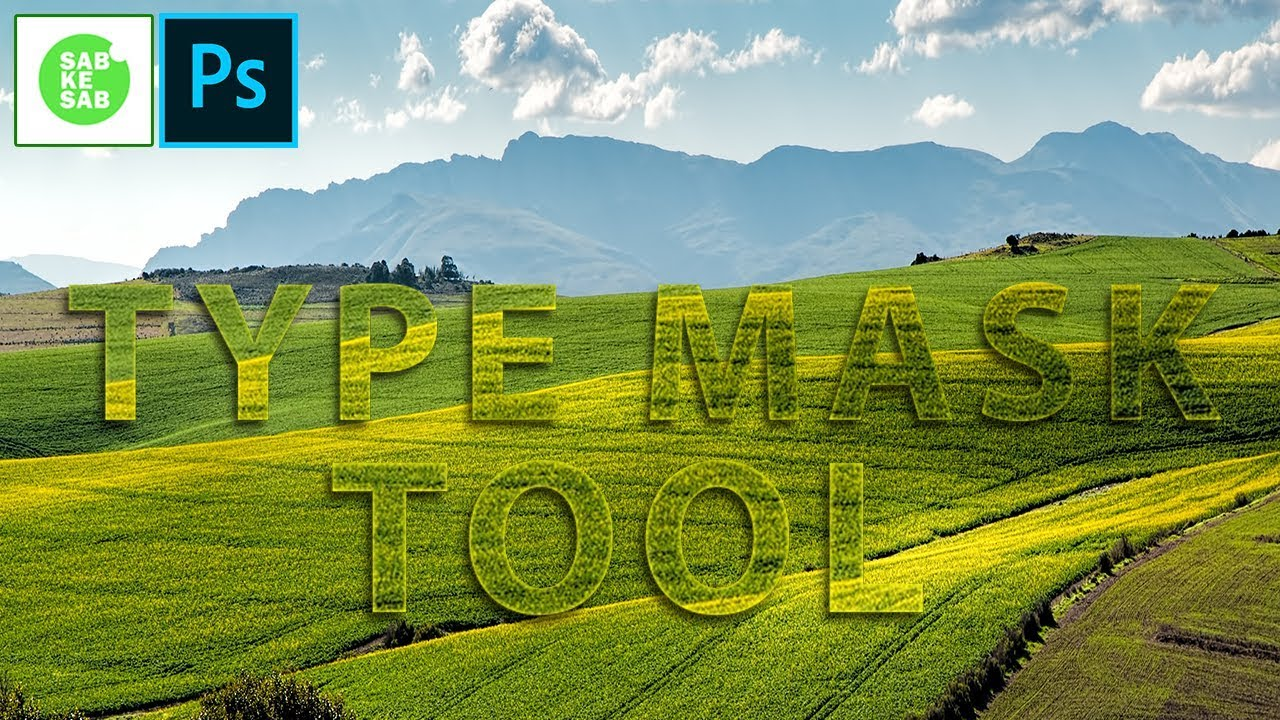
\includegraphics[width = 0.9\textwidth]{images/maxresdefault (1).jpg}
	\end{center}
\end{frame}

		\subsection{Editing Text}
\begin{frame}
	\frametitle{Transformations}
	\begin{itemize}
		\item You can use all of the Transform tools on Type.
		\item This will allow you to scale, warp and distort text in any way you want.
	\end{itemize}
	\begin{center}
		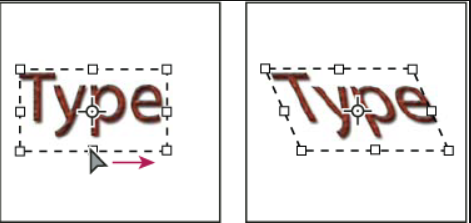
\includegraphics[width = 1.0\textwidth]{images/type transform.png}
	\end{center}
\end{frame}

\begin{frame}
	\frametitle{Character Panel}
	\begin{columns}
		\column{.5\textwidth}
	\begin{itemize}
		\item Font Type
		\item Bold, Italics, Regular
		\item Font Size
	\end{itemize}
\column{.5\textwidth}
	\begin{itemize}
	\item Space between lines
	\item Font Colour
	\item Scale
\end{itemize}
\end{columns}
	\begin{center}
		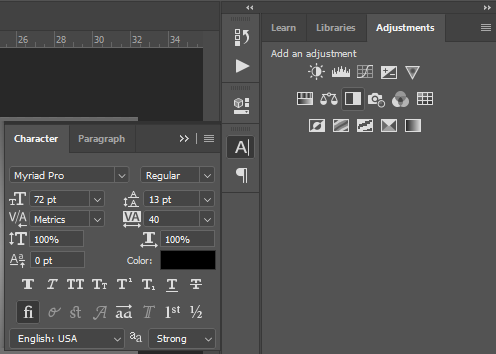
\includegraphics[width = 0.75\textwidth]{images/character panel.png}
	\end{center}
\end{frame}

\begin{frame}
	\frametitle{Paragraph Panel}
	\begin{itemize}
		\item Alignment (left, right, center, justified)
		\item Indentations
		\item First/Last line indents
	\end{itemize}
	\begin{center}
		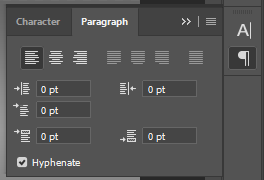
\includegraphics[width = 0.75\textwidth]{images/paragraph panel.png}
	\end{center}
\end{frame}
		
		
	\section{Layer Styles}
		\begin{frame}
		\frametitle{Fill and Adjustment Layers}
		\begin{center}
			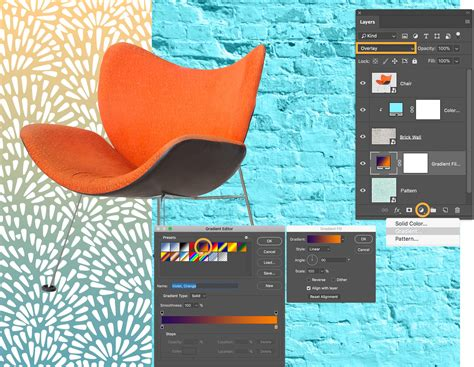
\includegraphics[width = 0.8\textwidth]{images/adjust and fill layers.jpg}
		\end{center}
	\end{frame}
	
	\subsection{What are Blending Options?}
	\begin{frame}
		\frametitle{What are Blending Options?}
		\begin{itemize}
			\item Layer styles let you quickly apply effects to an entire layer.
			\item In the Effects panel, you can view a variety of predefined layer styles and apply a style with just a click of the mouse.
			\item Layer effects are linked to the layer contents.
			\item You can apply multiple effects in a single layer style. Also, more than one instance of some effects can comprise a layer style.
		\end{itemize}
		\begin{center}
			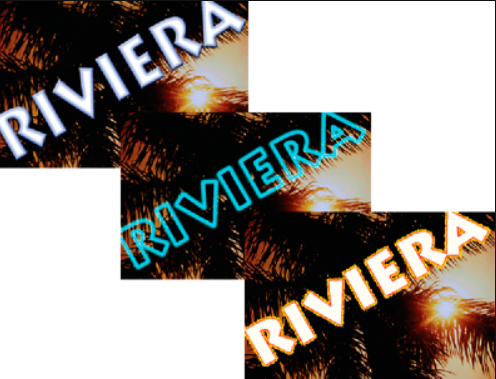
\includegraphics[width = 0.5\textwidth]{images/layer styles.png}
		\end{center}
	\end{frame}
	
	\subsection{How to access Blending Options?}
	\begin{frame}
		\frametitle{How to access Blending Options?}
				\begin{columns}
			\column{.6\textwidth}
			\vspace{-15pt}
		\begin{outline}
			\1 Right click on the layer which you want to edit.
			\1 Click on Blending Options...
		\end{outline}
	\column{.4\textwidth}
		\begin{center}
			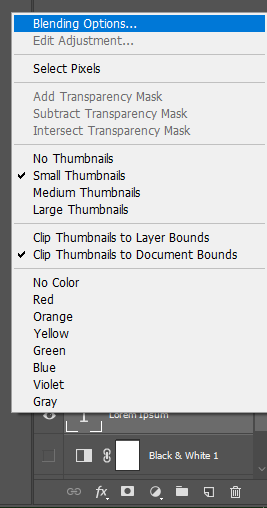
\includegraphics[width = 0.8\textwidth]{images/blending options.png}
		\end{center}
	\end{columns}
	\end{frame}

	\subsection{What do they do?}
	\begin{frame}
	\frametitle{What does each Blending Option do?}
	\begin{outline}
		\1 Bevel \& Emboss - Add various combinations of highlights and shadows to a layer.
		\1 Stroke - Outlines the object on the current layer using color, a gradient, or a pattern. It is particularly useful on hard-edged shapes such as type.
		\1 Inner Shadow - Adds a shadow that falls just inside the edges of the layer's content, giving the layer a recessed appearance.
		\1 Inner Glow - Adds glow from the inside edges of the layer.
		\1 Satin - Applies interior shading that creates a satiny finish.
		\1 Color Overlay - Fills the layer's content with a color.
		\1 Gradient Overlay - Fills the layer's content with a gradient.
		\1 Pattern Overlay - Fills the layer's content with a pattern.
		\1 Outer Glow - Add glows that emanate from the outside edges of the layer's content.
		\1 Drop Shadow - Adds a shadow that falls behind the layer.
	\end{outline}
\end{frame}

\subsection{Show/Hide Effects}
	\begin{frame}
	\frametitle{How to view and hide Effects}
	\begin{itemize}
		\item Click the eye icons to hide and show each individual layer style.
	\end{itemize}
	\begin{center}
			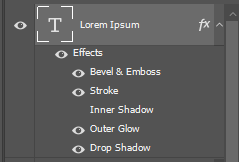
\includegraphics[width = 0.5\textwidth]{images/effects3.png}
	\end{center}
\end{frame}

	\begin{frame}
	\frametitle{How to view and hide Effects in Layers Tab}
	\begin{itemize}
		\item You can view and hide the layer styles applied to each layer.
		\item Click the drop down array next to the fx symbol
	\end{itemize}
	\begin{center}
		\begin{columns}
			\column{.5\textwidth}
		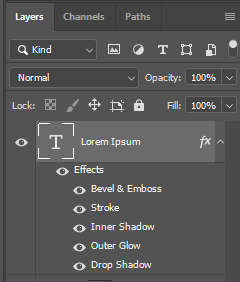
\includegraphics[width = 0.5\textwidth]{images/effects.png}
		\column{.5\textwidth}
		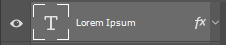
\includegraphics[width = 0.5\textwidth]{images/effects2.png}
	\end{columns}
	\end{center}
\end{frame}

	\begin{frame}
	\frametitle{How to disable effects}
	\begin{itemize}
		\item Right click the Effects
		\item Select "Disable Layer Effects"
	\end{itemize}
	\begin{center}
		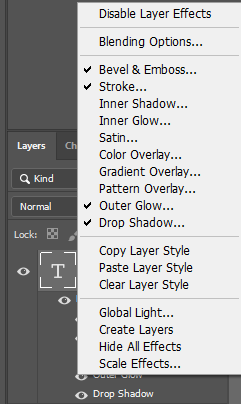
\includegraphics[width = 0.5\textwidth]{images/disable effects.png}
	\end{center}
\end{frame}

\subsection{Copy/Paste Effects}
\begin{frame}
	\frametitle{How to Copy and Paste Effects}
			\begin{columns}
				\column{.5\textwidth}
	\begin{itemize}
		\item Right-click on the effects you wish to copy
		\item Select "Copy Layer Style"
		\item Then Right-click on the layer you wish to paste the style to
		\item Select "Paste Layer Style"
	\end{itemize}
\column{.5\textwidth}
	\begin{center}
			
			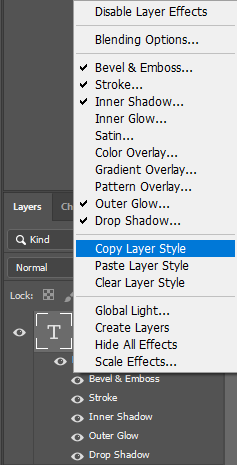
\includegraphics[width = 0.5\textwidth]{images/copy layer style.png}
	\end{center}
	\end{columns}
\end{frame}

	\section{The Snipping Tool}	
		\begin{frame}
		\frametitle{The Snipping Tool}
		\begin{center}
			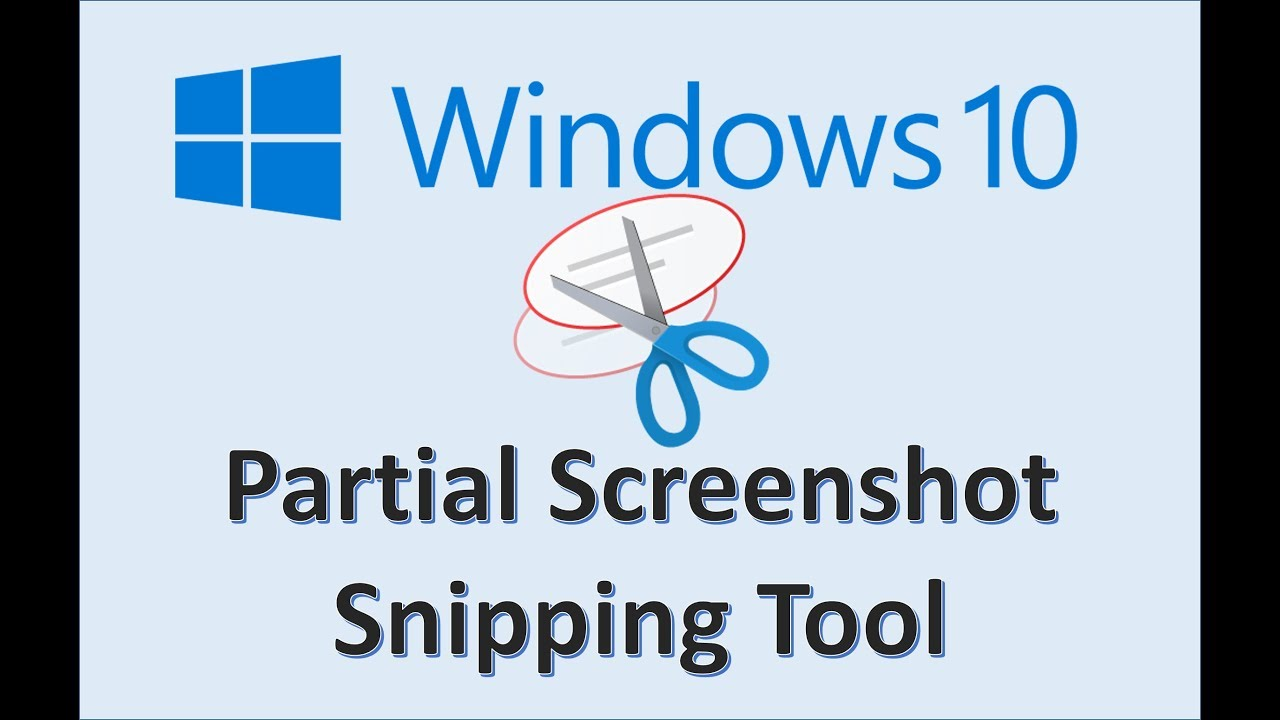
\includegraphics[width = 0.8\textwidth]{images/maxresdefault (2).jpg}
		\end{center}
	\end{frame}
	
	\subsection{What is the Snipping Tool}
	\begin{frame}
		\frametitle{What is the Snipping Tool?}
		\begin{outline}
			\1 It can take still screenshots of an open window, rectangular areas, a free-form area, or the entire screen. 
			\1 Snipping Tool allows for basic image editing of the snapshot, with different colored pens, an eraser, and a highlighter.
			\1 Snips can be stored as an image file (PNG, GIF, or JPEG).
		\end{outline}
		\begin{center}
			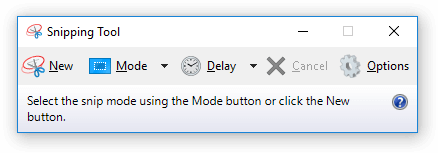
\includegraphics[width = 1.0\textwidth]{images/snipping-tool.png}
		\end{center}
	\end{frame}

\subsection{How to use the Snipping Tool}
	\begin{frame}
	\frametitle{How to use the Snipping Tool?}
	\begin{outline}
		\1 Search Snipping Tool in the Windows Task Bar, and open it
		\1 Click "New" and then Click and Drag to select the area to take a screen shot of.
	\end{outline}
	\begin{center}
		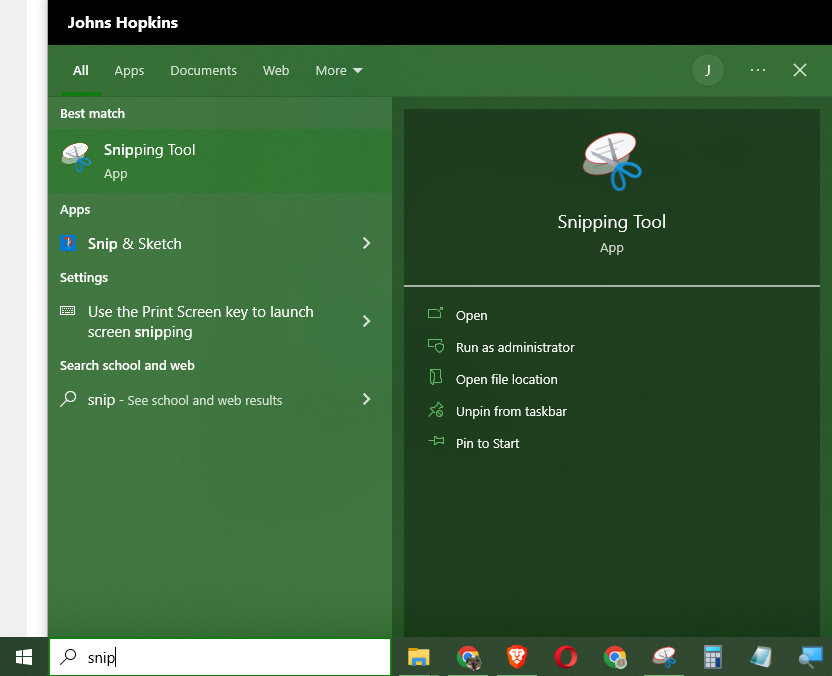
\includegraphics[width = 0.75\textwidth]{images/using snipping tool.png}
	\end{center}
\end{frame}

	\section{}	
		\subsection{End Card}
	\begin{frame}
		\frametitle{End Card}	
		\begin{columns}
			\column{.6\textwidth}
			\vspace{-25pt}
			\begin{itemize}
				\item Joshua Paul Barnard
				\item Computer Science Instructor
				\item Mendocino College
			\end{itemize}
			\begin{itemize}
				\item This Presentation was made in \LaTeX
				\item For the Fall 2022 semester.  
			\end{itemize}
			\begin{itemize}
				\item jbarnard@mendocino.edu
				\item github.com/JoshuaPaulBarnard
			\end{itemize}
			\column{.45\textwidth}
			
\includegraphics[width=.85\textwidth]{images/shone farm wine pouring - vert.png}
		\end{columns}
	\end{frame}
	
\end{document}